\newpage
\section{Datenvisualisierung}\label{sec:Datenvisualisierung}
Die Visualisierung der aufgezeichneten Messwerte sowie der ermittelten Zustandsbewertung des Systems soll über die Open-Source-Software Grafana erfolgen. Die Visualisierung der Daten soll hierbei nicht an die Zielplattform gebunden sein und von jedem beliebigen Rechner abrufbar sein. Des Weiteren soll die Möglichkeit geboten sein, die Werte verschiedener Plattformen in einem gemeinsamen Dashboard anzeigen zu lassen.\\
Das Konzept für eine Plattformunabhängige Visualisierung der Hardware-Health-Monitoring Daten wird in Abbildung \ref{fig:DatenvisualisierungKonzept} gezeigt. Hierbei werden die Daten der einzelnen Zielplattformen, einem zentralen Server über eine \ac{api} in der Anwendung bereitgestellt. Der Grafana Service wird anschließend von einem separaten Server dem Anwender bereitgestellt.   
\begin{center}
    \begin{figure}[h!]
        \captionsetup{justification=centering,format=plain, font=small}
        \centering
        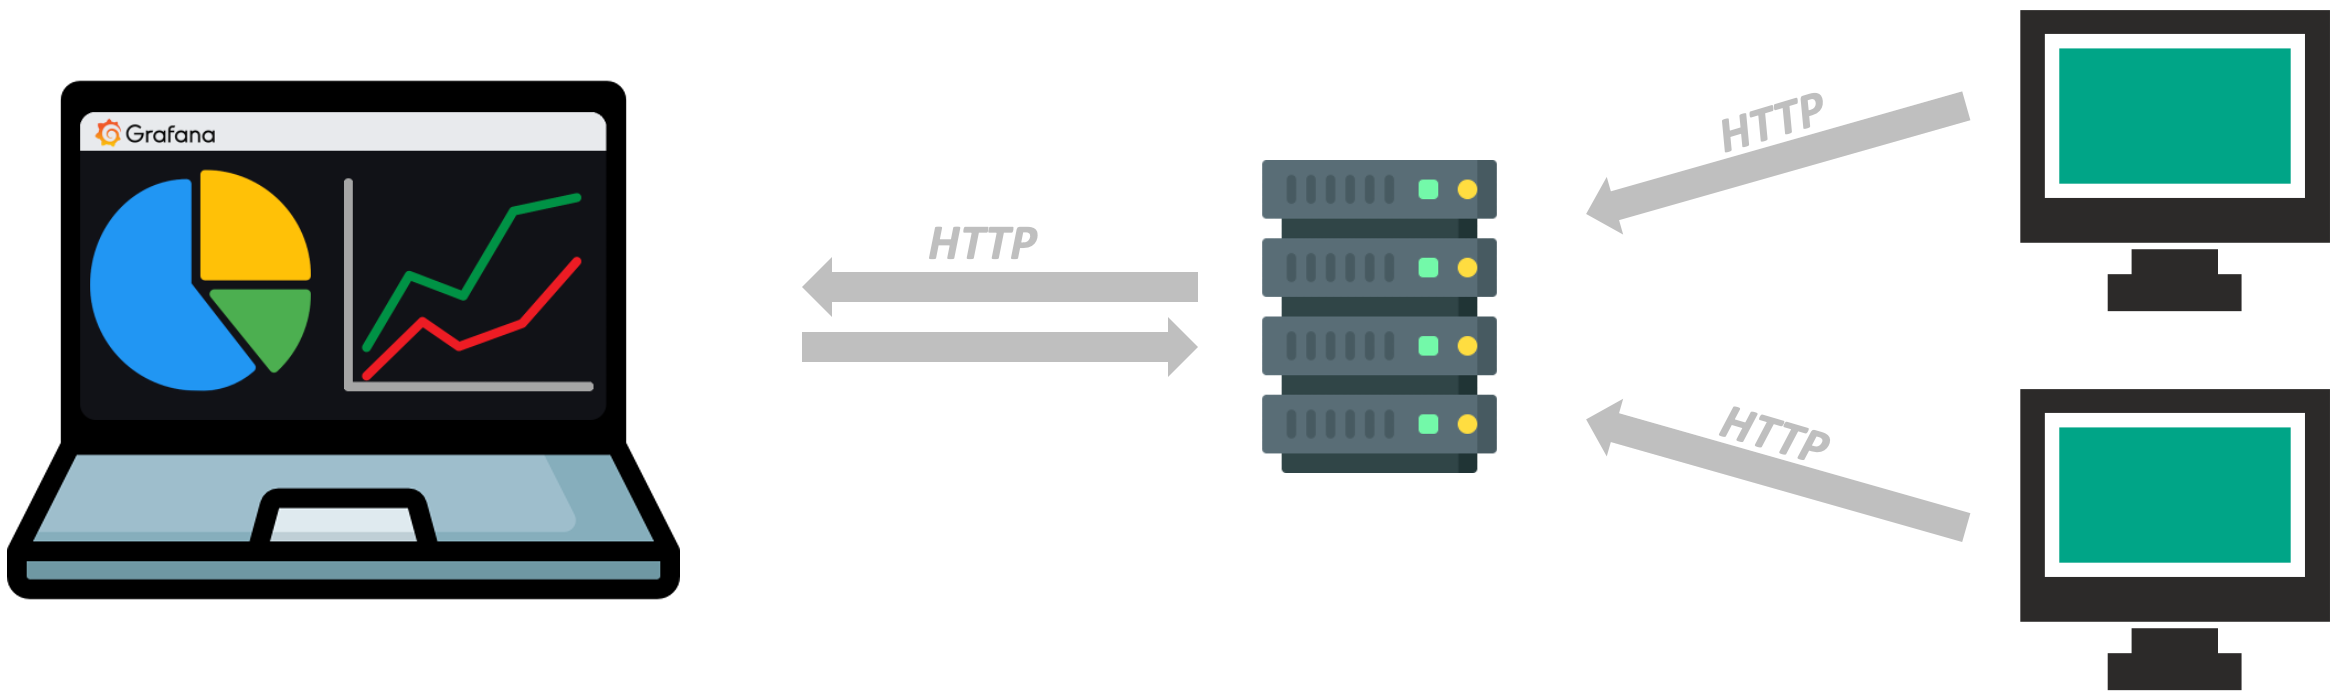
\includegraphics[width=1\textwidth]{Datenvisualisierung.png}
        \caption{Konzept zur Platformunabhängigen Datenvisualisierung}
        \label{fig:DatenvisualisierungKonzept}
    \end{figure}
\end{center}

\subsection{Architektur der REST API}
Die in Grafana verwendete Datenquelle \textit{SimpleJSON} diktiert die Struktur der \ac{api}. In der Dokumentation der Datenquelle \cite{SimpleJSON} werden die URL Pfade so wie Body der \acs{http} Anfragen erläutert.\\
Hierbei können, nach Abbildung \ref{fig:APIAnfragen}, die \ac{http} Anfragen an drei URL-Pfade gesendet werden. Die URL mit dem Ende \glqq\textit{/}\grqq{} wird zum Testen der Verbindung genutzt. Anfragen an die URL \glqq\textit{/search}\grqq{} liefern eine Liste an vorhandenen Datensätze zurück. Diese wird genutzt, um einen bestimmten Datensatz mit dem nächsten Aufruf der \ac{api} anzufragen. Über eine Anfrage an \glqq\textit{/query}\grqq{} können die gewünschten Datensätze erhalten werden.\\
\begin{center}
    \begin{figure}[h!]
        \captionsetup{justification=centering,format=plain, font=small}
        \centering
        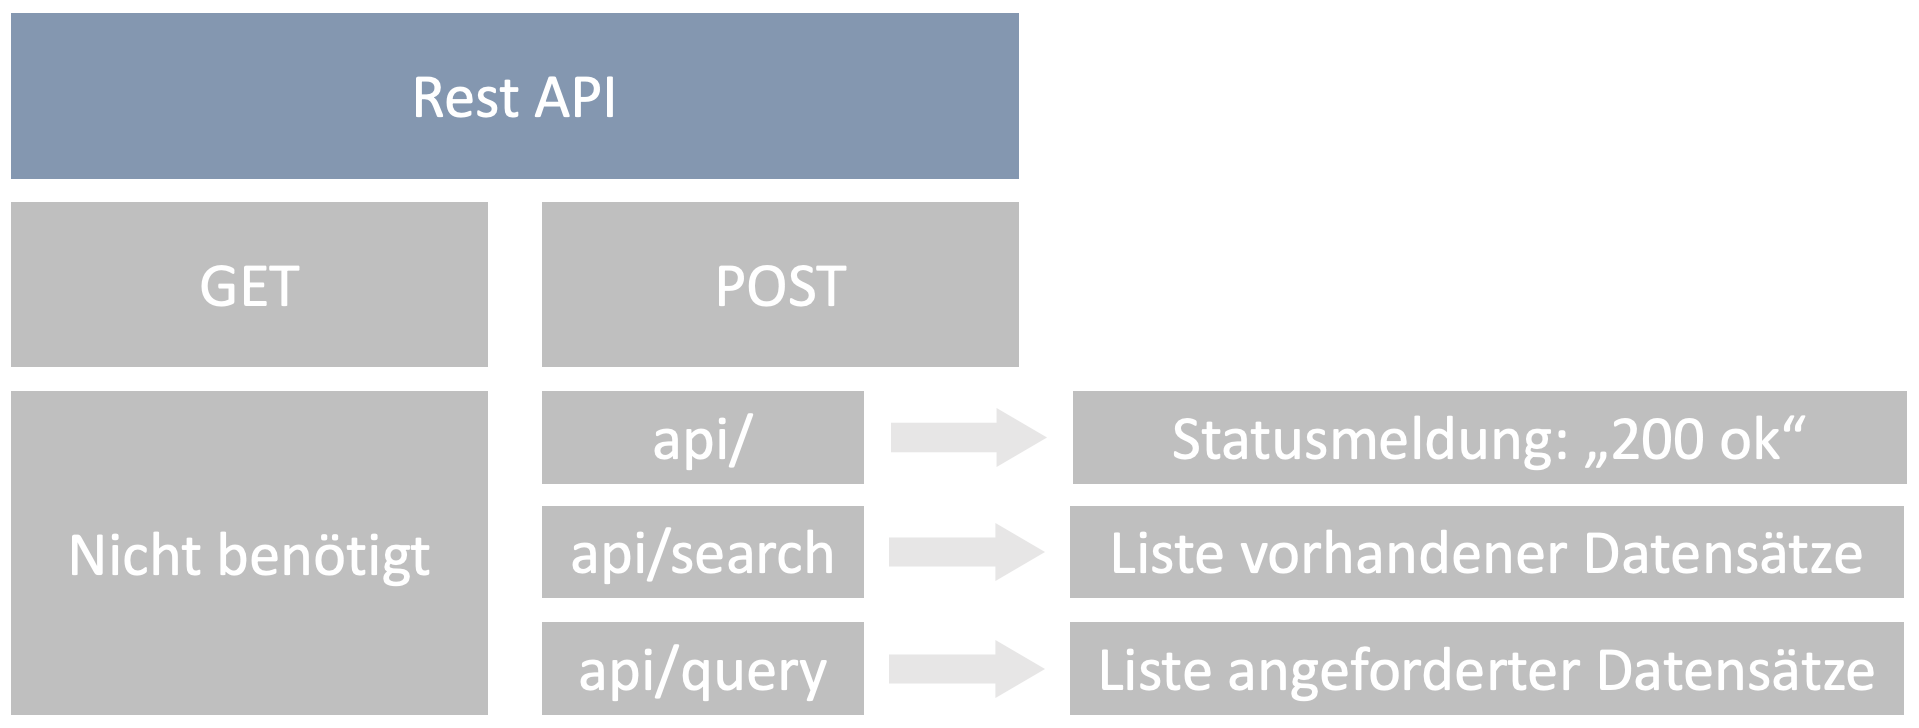
\includegraphics[width=1\textwidth]{APIAufrufe.png}
        \caption{Visualisierung der \ac{http} Anfragen an die \ac{api}}
        \label{fig:APIAnfragen}
    \end{figure}
\end{center}
\vspace{-1.8cm}
Da die Anfragen von Grafana in zufälligen Intervallen gestellt werden, muss die \ac{api} zu jedem beliebigen Zeitpunkt auf diese reagieren können. Um während der Behandlung einer Anfrage, nicht das gesamte Programm lahm zu legen, wird die \ac{api} des Hardware Health Monitors in einem separaten Thread gestartet und läuft unabhängig vom in Abschnitt \ref{sec:Gesamtkonzept} behandelten Taskscheduler.\\
Die \ac{api} wird in der Architektur der gesamten Anwendung von einer einfachen Klasse, welche unter dem Verzeichnis \textit{HM.API} organisiert ist, repräsentiert. Abbildung \ref{fig:UMLAPI} zeigt zudem die verwendeten Ressourcen der Schnittstelle. 
\begin{center}
    \begin{figure}[h!]
        \centering
        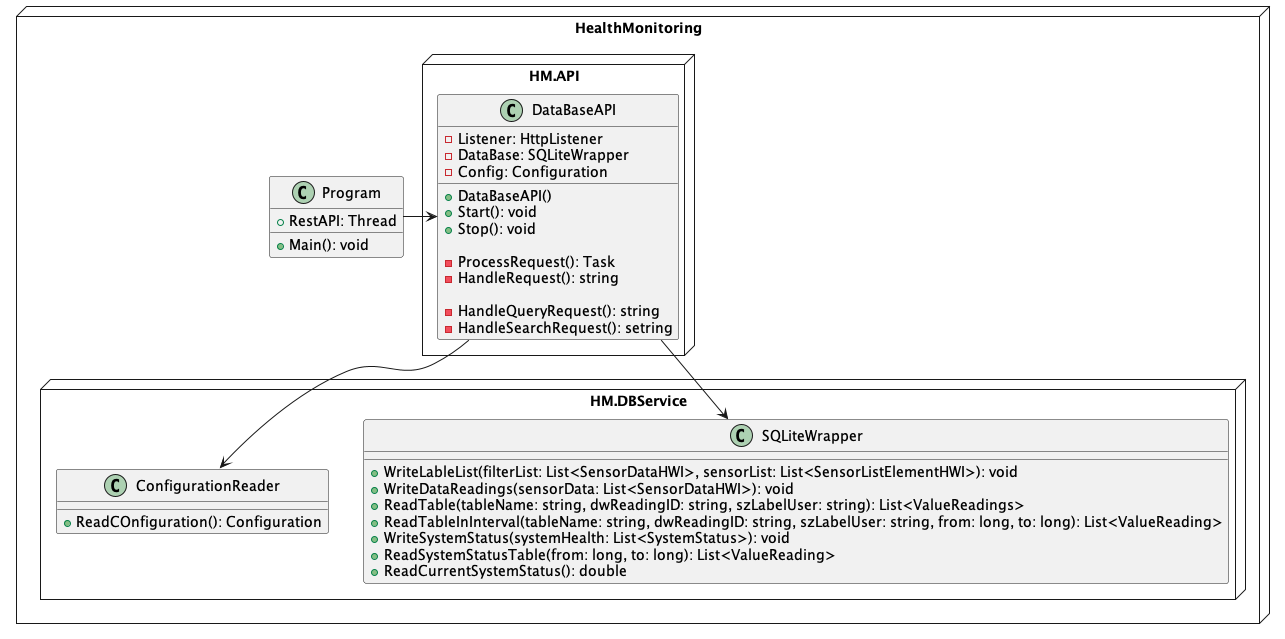
\includegraphics[width=1\textwidth]{DataBaseAPI.png}
        \caption{Arichtektur der \ac{api}}
        \label{fig:UMLAPI}
    \end{figure}
\end{center}
\vspace{-1.8cm}